\documentclass{article}

% ---------------------------------------------------------------------------
% Course template, anonymous submission version.
% The default option set of ai4science_ysda2026 prints "Anonymous authors",
% hides affiliations, correspondence and acknowledgements, and leaves the PDF
% author field empty; there is no local switch for this. The final version is
% produced by the author with the [final] option, which is not used here.
% The course style is checked in alongside this source when the paper is saved.
% ---------------------------------------------------------------------------
\usepackage[english]{ai4science_ysda2026}

\usepackage{amsmath,amssymb}
\usepackage{booktabs}
\usepackage{graphicx}
\usepackage{microtype}
\graphicspath{{./}{../experiment/results/}}
\setlength{\dbltextfloatsep}{10pt plus 2pt minus 2pt}

% Generated by experiment/make_paper_numbers.py from
% experiment/results/summary.json and experiment/results/paired_errors.csv.
% Do not edit by hand: rerun the script instead.
\newcommand{\NScenes}{25}
\newcommand{\MeanDiff}{10.66}
\newcommand{\MeanDiffSigned}{+10.66}
\newcommand{\CILow}{3.59}
\newcommand{\CIHigh}{17.09}
\newcommand{\MedianDL}{8.04}
\newcommand{\MedianGauss}{18.60}
\newcommand{\CountDL}{21}
\newcommand{\CountGauss}{14}
\newcommand{\ThresholdM}{20}
\newcommand{\NResamples}{10{,}000}
\newcommand{\BootstrapSeed}{20261121}
\newcommand{\NPositive}{22}
\newcommand{\NNegative}{3}
\newcommand{\MaxDiff}{43.77}
\newcommand{\MaxDiffScene}{168}
\newcommand{\MinDiff}{40.78}
\newcommand{\MinDiffScene}{167}
\newcommand{\MaxErrDL}{55.45}
\newcommand{\MaxErrDLScene}{167}
\newcommand{\MaxErrGauss}{74.25}
\newcommand{\MaxErrGaussScene}{164}
\newcommand{\PythonVersion}{3.14.4}
\newcommand{\NumpyVersion}{2.5.4}
\newcommand{\MatplotlibVersion}{3.11.2}


\icmltitlerunning{Predicting the Concentration-Weighted Plume Center}

\begin{document}

\twocolumn[

  \icmltitle{Predicting the Concentration-Weighted Center of\\
    Urban Pollutant Plumes: A Comparison of a Gaussian Model\\
    and a Deep Learning Model}

  \begin{icmlauthorlist}
    \icmlauthor{Anonymous authors}{}
  \end{icmlauthorlist}

  \icmlkeywords{urban dispersion, concentration-weighted plume center,
    deep learning surrogate, Gaussian model, large-eddy simulation}

  \vskip 0.1in
]

\printAffiliationsAndNotice{}
\setlength{\parskip}{4pt}

\begin{abstract}
The concentration-weighted mean of the grid-cell coordinates summarizes where
a plume lies. We compare a simplified stationary Gaussian plume model with
Briggs dispersion widths and a U-Net surrogate trained on large-eddy
simulation (LES) concentration fields. For each of \NScenes{} urban layouts,
we measure the distance from each model's plume center to the LES plume
center at 3\,m above ground. The U-Net error is \MeanDiff\,m smaller on
average, and the U-Net center is closer to the LES center on \NPositive{} of
\NScenes{} layouts.
\end{abstract}

\section{Introduction}
\label{sec:intro}

Deep learning surrogates offer a computationally cheaper way to estimate
urban dispersion fields than large-eddy simulation. Aggregate pointwise
scores can obscure a displacement of the plume. The concentration-weighted
plume center provides a direct measure of its position.

We compare how closely a U-Net surrogate and a stationary Gaussian baseline locate the LES plume center. Within each layout, we calculate all three plume centers using the same set of valid cells, defined as grid cells outside buildings at 3 m above ground.

Mendil et al. compared a deep learning surrogate with a Gaussian model
for emergency pollution forecasting in an urban setting
\citep[\S2.3.2--2.3.3 and \S4.2]{mendil2022}. Here we compare plume center
errors for road emissions on a fixed archive of layouts and check the center calculation against synthetic fields with known centers.

\begin{figure*}[t]
  \centering
  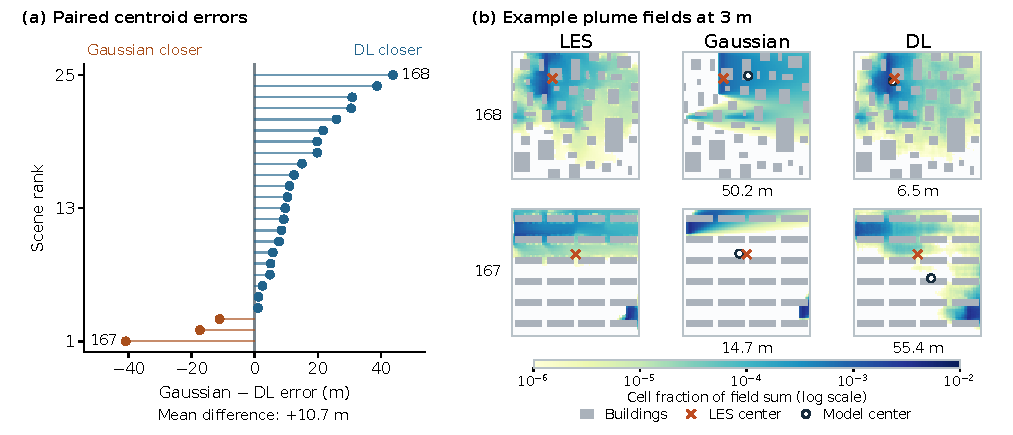
\includegraphics[width=0.70\textwidth]{paper_figure.pdf}
  \caption{(a) Sorted paired differences in plume center error, one point per layout. Positive differences favor the U-Net. (b) LES, Gaussian and U-Net fields at 3\,m for the two layouts with the largest differences in
    opposite directions. Crosses mark LES centers and circles mark model centers. The shared logarithmic scale shows each cell's fraction of the concentration summed over valid cells.}
  \label{fig:paired}
\end{figure*}

\section{Methods}
\label{sec:methods}

\subsection{Data and design}

We use steady-state pollutant concentration fields for \NScenes{} synthetic
urban layouts. The LES domain measures \mbox{$256 \times 256 \times 160$\,m},
with a horizontal grid spacing of 2\,m. A prescribed horizontal pressure
gradient drives the wind. Each layout can contain several road emission
sources, modeled as elongated boxes 8\,m high. We compare the fields on a
two-dimensional horizontal slice at 3\,m above ground, using only cells
outside buildings.

\subsection{Gaussian baseline}

We use a simplified ISC3-based stationary Gaussian model with ground
reflection \citep[\S1.1.1, Eq.~(1-1), and \S1.1.6.1, Eq.~(1-50)]{epa1995}.
Each road source is divided along grid-cell boundaries, and its emission is
distributed among the resulting elements in proportion to their areas
\citep[\S1.2.3]{epa1995}. Each element contributes a point kernel at its center.

For element $s$ with relative emission $Q_s$, let $a_s$ and $b_s$ denote
the downwind and crosswind distances from its center to the receptor.
Transport is directed opposite to the horizontal pressure gradient. The
model sums the kernels $C_s$ over the elements. A common wind-speed
factor cancels in the center calculation. For $a_s>0$,
\begin{equation}
  \begin{aligned}
    C_s &= \frac{Q_s}{2\pi\sigma_y\sigma_z}
          \exp\!\left(-\frac{b_s^2}{2\sigma_y^2}\right) \\
        &\quad \times \sum_{k\in\{-1,1\}}
          \exp\!\left(-\frac{(z_r-kz_s)^2}{2\sigma_z^2}\right).
  \end{aligned}
  \label{eq:gaussian}
\end{equation}
The receptor is at $z_r=3$\,m, and the 0--8\,m release layer is represented
at $z_s=4$\,m. The term for $k=-1$ accounts for ground reflection. For
$a_s\leq0$, $C_s=0$. The urban Briggs widths for neutral class~D
\citep[App.~D]{briggs1973}
\citep[\S1.1.5.1, Tables 1-3 and 1-4]{epa1995} are
\begin{equation}
  \sigma_y=\frac{0.16a}{\sqrt{1+0.0004a}},\qquad
  \sigma_z=\frac{0.14a}{\sqrt{1+0.0003a}},
  \label{eq:widths}
\end{equation}
where $a=\max(a_s,1\,\mathrm{m})$ and distances are in meters.

\subsection{Plume center and error}

Let $M$ be the set of cells outside buildings at 3\,m. For a concentration
field $c_{ij}$, the plume center is the weighted mean of the cell centers,
\begin{equation}
  \begin{aligned}
    x_c &= \frac{\sum_{(i,j)\in M} c_{ij}\,x_{ij}}
                {\sum_{(i,j)\in M} c_{ij}}, \\
    y_c &= \frac{\sum_{(i,j)\in M} c_{ij}\,y_{ij}}
                {\sum_{(i,j)\in M} c_{ij}},
  \end{aligned}
  \label{eq:centroid}
\end{equation}
with $x_{ij}=(j+\tfrac12)\cdot2$\,m and $y_{ij}=(i+\tfrac12)\cdot2$\,m, applied to
LES and to both models. For model $m$ the error is the Euclidean distance to the
LES plume center,
\begin{equation}
  e_m = \sqrt{\left(x_c^{\mathrm{LES}} - x_c^{m}\right)^2
            + \left(y_c^{\mathrm{LES}} - y_c^{m}\right)^2}.
  \label{eq:error}
\end{equation}

\subsection{Paired comparison}

Both models are evaluated on the same scenes, and the paired difference is
\begin{equation}
  d_g = e_{\mathrm{Gaussian},g} - e_{\mathrm{DL},g},
  \label{eq:paired}
\end{equation}
so that positive values indicate a smaller U-Net error. We summarize the
comparison by the mean of $d_g$, the number of layouts favoring each model
and the median error for each model.

\subsection{Verification and reproduction}

We test the plume center calculation on synthetic fields with known
centers. If only one cell has a nonzero concentration, the calculated
plume center must coincide with the center of that cell. To check the
building mask, we start with a uniform patch centered at $(90,70)$\,m.
We add a high-concentration cell outside the patch and mark it as a
building cell. The calculation should still return $(90,70)$\,m.
Finally, we shift a test field one grid cell to the right and check
that its calculated center moves exactly 2\,m in the same direction.

To reproduce the comparison, we use the archived LES and U-Net fields
and recompute the Gaussian fields from the saved road sources and
pressure gradients. We then calculate the three plume centers using
the same building mask for each layout.


\section{Results}
\label{sec:results}

Figure~\ref{fig:paired}(a) shows one point per layout. The horizontal
axis gives the Gaussian error minus the U-Net error, and the vertical
axis ranks the layouts by this difference. Points to the right of zero
indicate that the U-Net placed the plume center closer to the LES
center. Points to the left indicate that the Gaussian model was closer.

Panel~(b) shows the LES, Gaussian and U-Net concentration fields at
3\,m above ground for the layouts at either end of the ranking.
The cross marks the LES plume center, and the circle marks the
predicted center. The distance between these markers is the error
printed below each model map. On layout~\MaxDiffScene{}, the U-Net
center is 6.5\,m from the LES center, compared with 50.2\,m for the
Gaussian model. On layout~\MinDiffScene{}, the Gaussian center is
14.7\,m from the LES center and the U-Net center is 55.4\,m away.

Across all \NScenes{} layouts, the U-Net error is \MeanDiff\,m smaller
on average. The U-Net is closer to the LES center on \NPositive{}
layouts, and the Gaussian model is closer on \NNegative{}. The median
error is \MedianDL\,m for the U-Net and \MedianGauss\,m for the
Gaussian model.

\section{Conclusion}
\label{sec:conclusion}

The U-Net locates the LES plume center more accurately on average, with
some layouts favoring the Gaussian baseline. The comparison covers one wind
index, one tracer and one height, and uses LES as a numerical reference. It
applies to the chosen Gaussian parameterization and the archived U-Net
checkpoint \texttt{combined\_family\_ft\_best}. A small center error can
coexist with errors in plume spread or shape.

\clearpage
\begin{thebibliography}{9}

\bibitem{mendil2022}
Mendil, Leirens, Armand, and Duchenne (2022).
\emph{Hazardous atmospheric dispersion in urban areas: A Deep Learning
approach for emergency pollution forecast}. Environmental Modelling \&
Software, article 105387. DOI
\href{https://doi.org/10.1016/j.envsoft.2022.105387}{10.1016/j.envsoft.2022.105387}.
Sections 2.3.2--2.3.3 and 4.2.

\bibitem{briggs1973}
Briggs, G.~A. (1973).
\emph{Diffusion Estimation for Small Emissions. Preliminary Report}.
Air Resources Atmospheric Turbulence and Diffusion Laboratory, NOAA,
Oak Ridge, TN. TID-28289. DOI
\href{https://doi.org/10.2172/5118833}{10.2172/5118833}.
Appendices D and E.

\bibitem{epa1995}
US Environmental Protection Agency (1995).
\emph{User's Guide for the Industrial Source Complex (ISC3) Dispersion Models,
Volume II}. EPA-454/B-95-003b.
\href{https://gaftp.epa.gov/AIR/aqmg/SCRAM/models/other/isc3/isc3v2.pdf}{PDF:
isc3v2.pdf}.
Sections 1.1.1, 1.1.5.1, 1.1.6.1, 1.2.3; Eqs.~(1-1) and (1-50);
Tables 1-3 and 1-4.

\end{thebibliography}

\end{document}
